\documentclass{article}

\usepackage[provide=*, magyar]{babel}

\usepackage{graphicx}
\usepackage{tikz}
\usepackage{pgfplots}

\pgfplotsset{compat=1.18}
\usetikzlibrary{calc}
\usepackage{calc}

\usetikzlibrary {arrows.meta}
\usepgfplotslibrary{fillbetween}

\usepackage{pdfpages}

\usepackage{amsmath}
\usepackage{siunitx}
\usepackage{tabularx}
\usepackage{booktabs}
\usepackage[table]{xcolor}
\usepackage{multicol}

\newcommand{\siunit}[2]{
	\SI{#1}{[#2]}
}

\newcommand{\n}[1]{
	\siunit{#1}{\newton}
}
\newcommand{\nmm}[1]{
	\siunit{#1}{\newton\mm}
}
\newcommand{\kn}[1]{
	\siunit{#1}{\kilo\newton}
}
\newcommand{\knm}[1]{
	\siunit{#1}{\kilo\newton\meter}
}
\newcommand{\mpa}[1]{
	\siunit{#1}{\mega\pascal}
}

\newcommand{\equal}[2]{
	\sum{#1} := 0 = #2
}

\newcommand{\circled}[1]{
	\raisebox{.5pt}{\textcircled{\raisebox{-.9pt} {#1}}}
}


\title{Szilárdságtan HF2}
\date{\today}
\author{Vári Gergő}

%\pgfmathsetmacro\s{.002}

\pgfmathsetmacro\d{58}
\pgfmathsetmacro\ds{\d * \s * 50}

\pgfmathsetmacro\L{1500}
\pgfmathsetmacro\Ls{\L * \s}

\pgfmathsetmacro\h{2500}
\pgfmathsetmacro\hs{\h * \s}

\newcommand{\forcewidth}{2}
\newcommand{\forcelength}{1.5}

\newcommand{\structurecolor}{lightgray}
\newcommand{\coordcolor}{orange}
\newcommand{\normalforcecolor}{blue}
\newcommand{\sharedforcecolor}{red}
\newcommand{\reactionforcecolor}{violet}
\newcommand{\beamforcecolor}{olive}

\newcommand{\coords}{
	\coordinate (A) at (\Ls, 0);
	\coordinate (B) at (3 * \Ls, -\hs);
	\coordinate (C) at (3 * \Ls, 0);
}

\newcommand{\coordsize}{4pt}
\newcommand{\pointsone}{
	\fill[\coordcolor] (A) circle (\coordsize) node[below right] {$A$};
	\fill[\coordcolor] (C) circle (\coordsize) node[below right] {$C$};
}
\newcommand{\pointstwo}{
	\fill[\coordcolor] (B) circle (\coordsize) node[below right] {$B$};
	\fill[\coordcolor] (C) circle (\coordsize) node[below right] {$C$};
}
\newcommand{\points}{
	\pointsone
	\pointstwo
}

\newcommand{\beamone}{
	\draw[line width=\ds, \structurecolor] (0, 0) -- (A);
	\draw[line width=\ds, \structurecolor] (A) -- (C);
	\fill[\structurecolor] (C) circle (.1);
}

\newcommand{\beamtwo}{
	\fill[\structurecolor] (C) circle (.1);
	\draw[line width=\ds, \structurecolor] (C) -- (B);
}

\newcommand{\sizewidth}{.1}
\newcommand{\sizelength}{6}
\newcommand{\sizesone}{
	\draw[line width=\sizewidth] (0, 0) -- +(0, \sizelength * 0.35);
	\draw[line width=\sizewidth] (A) -- +(0, \sizelength * 0.35);
	\draw[line width=\sizewidth] (2 * \Ls, 0) -- +(0, \sizelength * 0.35);
	\draw[line width=\sizewidth] (C) -- +(0, \sizelength * 0.35);

        \draw[line width=\sizewidth, Stealth-Stealth, ]
                (0, \sizelength * 0.35) -- +(\Ls, 0)
                node[midway, above] {$L$};
        \draw[line width=\sizewidth, Stealth-Stealth, ]
                (\Ls, \sizelength * 0.35) -- +(\Ls, 0)
                node[midway, above] {$L$};
        \draw[line width=\sizewidth, Stealth-Stealth, ]
                (2 * \Ls, \sizelength * 0.35) -- +(\Ls, 0)
                node[midway, above] {$L$};

}
\newcommand{\sizestwo}{
	\draw[line width=\sizewidth] (C) -- +(\sizelength * 0.35, 0);
	\draw[line width=\sizewidth] (B) -- +(\sizelength * 0.35, 0);
        \draw[line width=\sizewidth, Stealth-Stealth, ]
                (3*\Ls + \sizelength * 0.35, 0) -- +(0, -\hs)
                node[midway, right] {$h$};
}
\newcommand{\sizes}{
	\sizesone
	\sizestwo
}
\newcommand{\sizepreview}{
	\draw[line width=\sizewidth, Bar-Bar] (10, 3) -- +(1000 * \s, 0) node[midway, above] {$\m{1}$};
}

\newcommand{\convention}{
        \draw[-Stealth] 
                (1.5 * \Ls + \Ls, 1.25 * \Ls) -- +(1, 0)
                node [below] {$x$};
        \draw[-Stealth] 
                (1.5 * \Ls + \Ls, 1.25 * \Ls) -- +(0, 1)
                node [left] {$y$};

        \draw[-Stealth]
		(2 * \Ls + \Ls, 1.25 * \Ls) arc (0:180:-.5)
                node [midway, above] {$+$};
}

\newcommand{\wholestructure}{
	\begin{figure}[hbt!]
		\centering
		\begin{tikzpicture}
			\coords
			
			\sizepreview
			\sizes

			\beamone
			\beamtwo

			\points
		\end{tikzpicture}
		\caption{Léptékhelyes ábra}
        \end{figure}
}

\newcommand{\normalforcesone}{
        \draw[line width=\forcewidth, \beamforcecolor, -Stealth] 
                (A) -- +(0, \forcelength)
                node[midway, left] {$A_z$};
        \draw[line width=\forcewidth, \beamforcecolor, -Stealth] 
		(2*\Ls, 0) -- +(0, -\forcelength)
                node[midway, right] {$F$};
		\draw[line width=\forcewidth * .5, \beamforcecolor, -Stealth] 
		(0, -.5) arc (90:-75:-.5) node[midway, left] {$M$};
}
\newcommand{\reactionforcesone}{
        \draw[line width=\forcewidth, \reactionforcecolor, -Stealth] 
		(C) -- +(0, \forcelength)
                node[midway, right] {$C_z$};
        \draw[line width=\forcewidth, \reactionforcecolor, -Stealth] 
		(C) -- +(\forcelength, 0)
                node[near end, below] {$C_x$};
}
\newcommand{\sharedforces}{
        \fill[\sharedforcecolor, opacity=.4] (2*\Ls, 0.1) rectangle +(\Ls, 1);
        \draw[line width=.2, \sharedforcecolor, -Stealth] 
                (2*\Ls + 1, \Ls * 0.25) -- +(0, -.5)
                node[midway, left] {$p$};

}

\newcommand{\normalforcestwo}{
	\draw[line width=\forcewidth * .5, \beamforcecolor, -Stealth] 
		(3*\Ls, -\hs +.5) arc (-90:90:-.5) node[near end, left] {$M^B$};
}
\newcommand{\reactionforcestwo}{
        \draw[line width=\forcewidth, \reactionforcecolor, -Stealth] 
		(3*\Ls, \forcelength) -- (C)
                node[midway, right] {$C_z$};
        \draw[line width=\forcewidth, \reactionforcecolor, -Stealth] 
		(C) -- +(-\forcelength, 0)
                node[near end, below] {$C_x$};
        \draw[line width=\forcewidth, \reactionforcecolor, -Stealth] 
		(B) -- +(\forcelength, 0)
                node[near end, below] {$B_x$};
        \draw[line width=\forcewidth, \reactionforcecolor, -Stealth] 
		(3*\Ls, -\hs - \forcelength) -- (B)
                node[near start, left] {$B_z$};
}

\newcommand{\forcesone}{
	\sharedforces
	\normalforcesone
	\reactionforcesone
}
\newcommand{\forcestwo}{
	\normalforcestwo
	\reactionforcestwo
}

\newcommand{\sztaone}{
	\begin{figure}[H]
		\centering
		\begin{tikzpicture}
			\coords

			\convention
			
			\sizesone

			\beamone
		
			\forcesone
			\pointsone
		\end{tikzpicture}
		\caption{1-es rúd SZTÁ}
        \end{figure}
}

\newcommand{\sztatwo}{
	\begin{figure}[H]
		\centering
		\begin{tikzpicture}
			\coords
			
			\sizestwo

			\beamtwo
		
			\forcestwo
			\pointstwo
		\end{tikzpicture}
		\caption{2-es rúd SZTÁ}
        \end{figure}
}
%

\begin{document}
	\pagenumbering{gobble}
	
	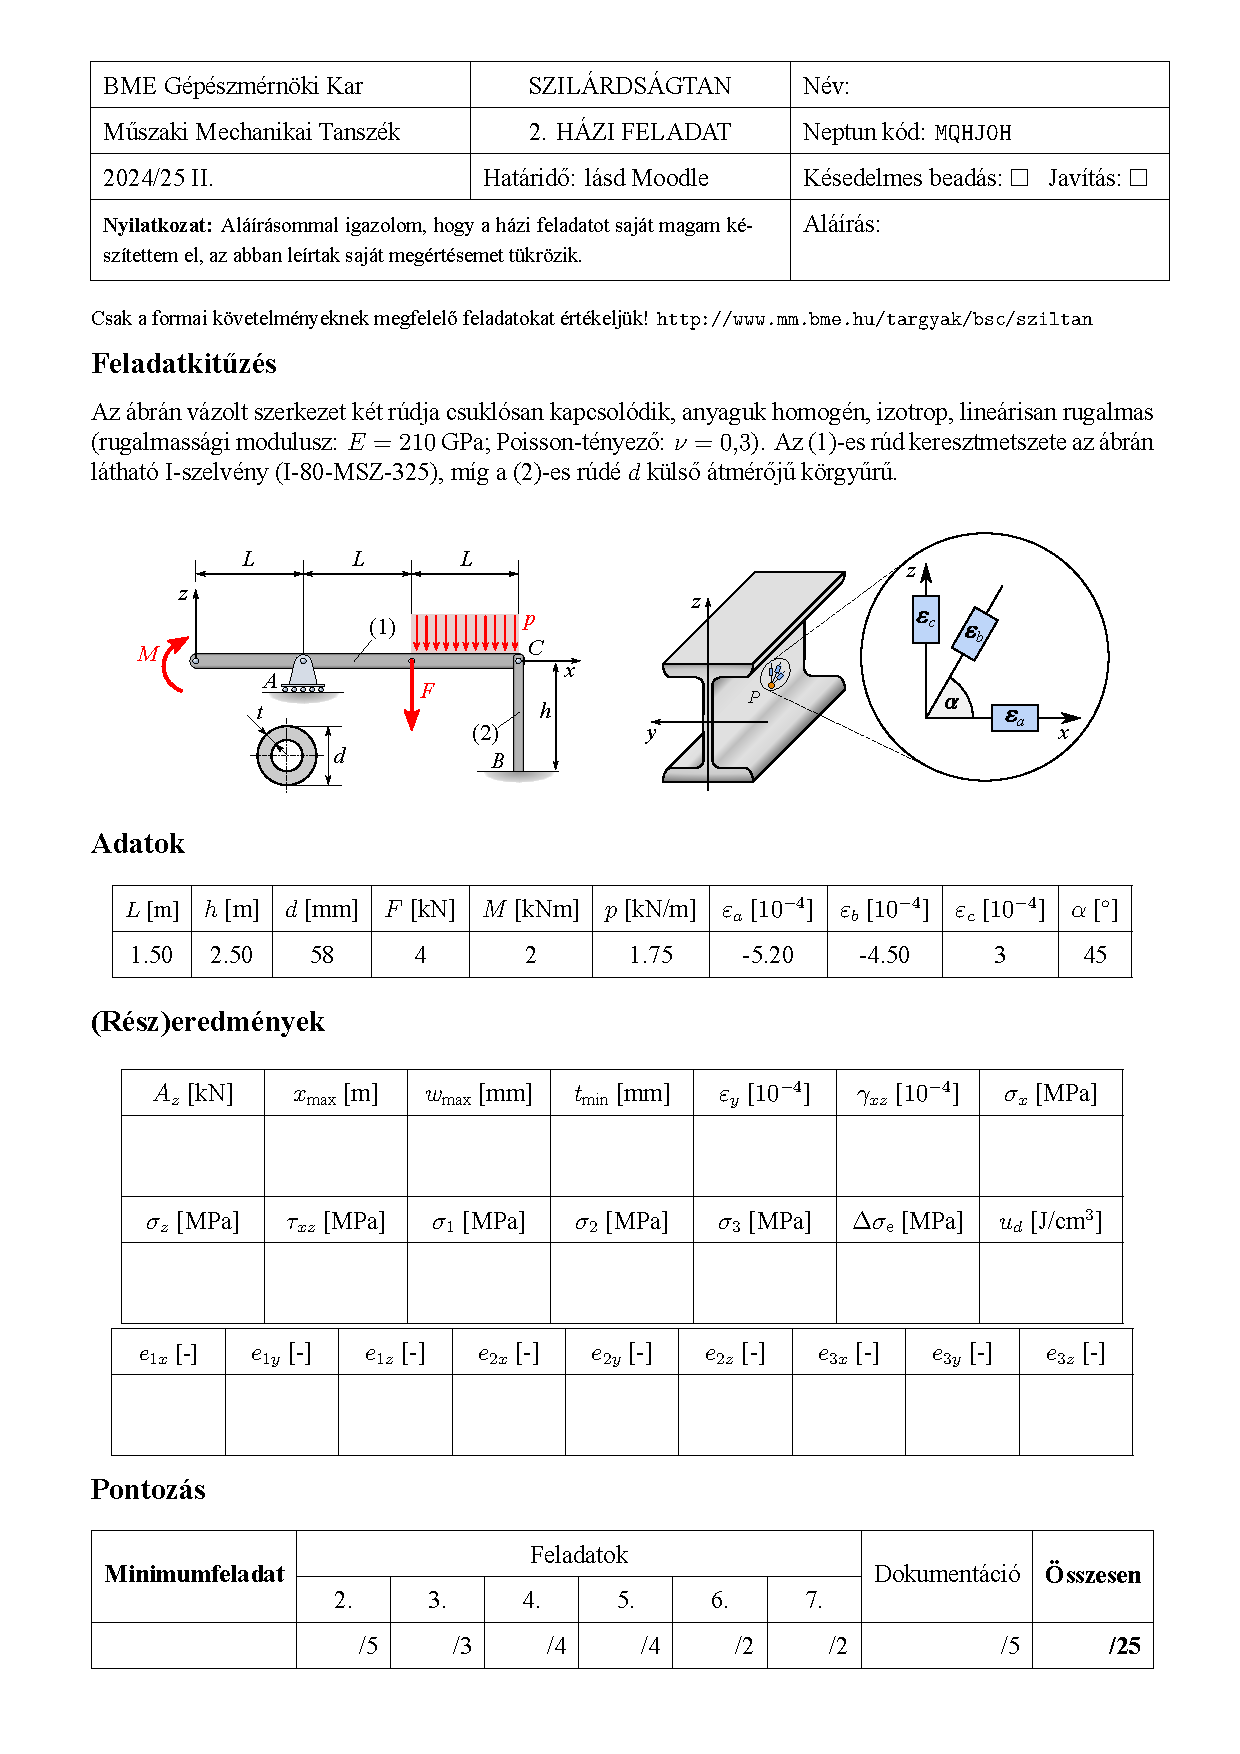
\includepdf[pages={1}, pagecommand={
	\begin{picture}(0,0) 
		\put(270, 93){Vári Gergő}
		{\fontfamily{cmr}\selectfont\put(290, 23){\Large{Vári Gergő}}}
		\put(-58, -393){\Large{1.98958}}
		\put(25, -393){\Large{0}}
		\put(75, -393){\Large{60.699}}
		\put(150, -393){\Large{2.5}}
		\put(208, -393){\Large{0.943}}
		\put(276, -393){\Large{-6.8}}
		\put(333, -393){\Large{-99.231}}
		\put(-55, -450){\Large{33.231}}
		\put(7, -450){\Large{-54.923}}
		\put(75, -450){\Large{53.041}}
		\put(155.5, -450){\Large{0}}
		\put(198, -450){\Large{-119.041}}
		\put(269, -450){\Large{19.445}}
		\put(337, -450){\Large{0.048}}
		\put(-67, -510){\Large{0.3393}}
		\put(0, -510){\Large{0}}
		\put(37, -510){\Large{-0.941}}
		\put(104, -510){\Large{0}}
		\put(155.5, -510){\Large{1}}
		\put(207, -510){\Large{0}}
		\put(247, -510){\Large{0.941}}
		\put(310, -510){\Large{0}}
		\put(346, -510){\Large{0.3393}}
	\end{picture}
}]{misc/exercise.pdf}


	\maketitle
	\rule{0pt}{50pt}
	\begin{figure}[hbt!]
		\centering
		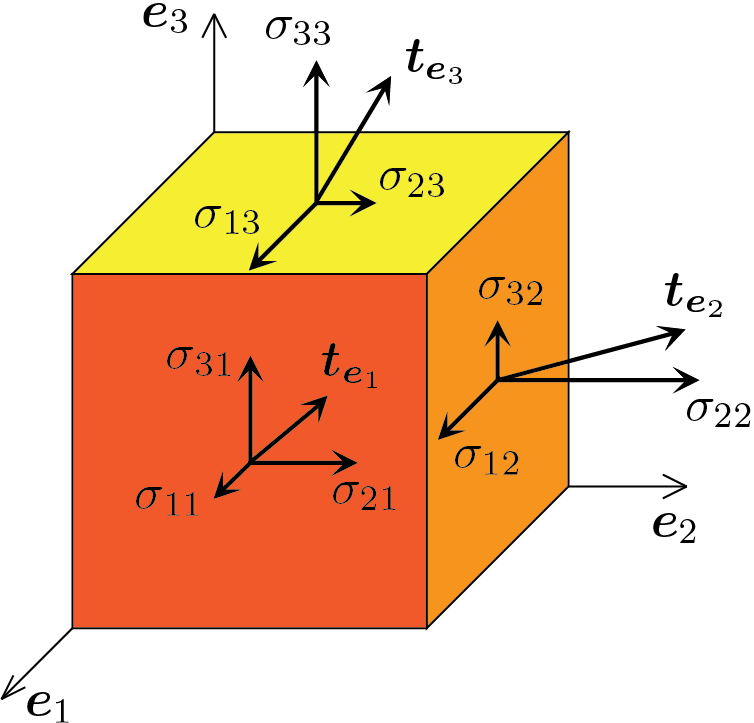
\includegraphics[scale=1.75]{./images/cauchy_stress_components.png}
		\caption{Cauchy feszültségi tenzor}
	\end{figure}

	\newpage
	\pagenumbering{arabic}
	
	\section{Reakció komponensek}

\wholestructure

\subsection{Egyensúlyi egyenletek}

\subsubsection{1-es rúd}

\sztaone

\begin{align*}
	&\equal{F_x}{C_x} \\
	&\equal{F_z}{A_z - F - pL + C_z} \\
	&\equal{M^A}{-M-F(L)-pL\left(\frac{3}{2}L\right)+C_z(2L)}
\end{align*}

\begin{align*}
	&A_z = \kn{1.98958} \\
	&C_x = \kn{0} \\
	&C_z = \kn{4.63542} 
\end{align*}

\subsubsection{2-es rúd}

\sztatwo

\begin{align*}
	&\equal{F_x}{-C_x+B_x} \\
	&\equal{F_z}{B_z - C_z} \\
	&\equal{M^B}{C_x(h)}
\end{align*}

\begin{align*}
	&B_x = C_x = \kn{0} \\
	&B_z = C_z = \kn{4.63542} 
\end{align*}

	\newpage

	\section{Lehajlásfüggvény}

\subsection{Hajlítónyomatéki igénybevételi függvény}
\newcommand{\mcolor}{cyan}
{\footnotesize
        \begin{center}
                \setlength{\aboverulesep}{0pt}
                \setlength{\belowrulesep}{0pt}
                \setlength{\extrarowheight}{.75ex}
		\begin{tabular}{rccc}
			\toprule
			\rowcolor{lightgray}
			$x$
			&$0 < x < L$
			&$L < x < L+R$
			&$L+R < x < 2L+R$ \\
			\toprule

			\rowcolor{\mcolor}
			$M_h$
			&$-M$
			&$-M-A_z(x-L)$ 
			&$-M-A_z(x-L)+F(x-2L)+p(x-2L)\frac{x-2L}{2}$ \\

			\bottomrule
		\end{tabular}
	\end{center}
}

\pgfmathsetmacro\M{2}
\pgfmathsetmacro\Az{1.98958}
\pgfmathsetmacro\p{1.75}
\pgfmathsetmacro\Cz{4.63542}

\begin{center}
	\begin{tikzpicture}
                \begin{axis}[
                        height={100},
                        width={272.5},
			xlabel={$x \m{}$},
                        ylabel={$M_h(x) \knm{}$},
                        axis lines=left,
                ]
                        \addplot [
                                domain=0:1.5,
                                \mcolor
                        ]
                                {-\M};
                        \addplot [
				domain=1.5:2*1.5,
                                \mcolor
                        ]
                                {-\M-\Az*(x-1.5)};
                        \addplot [
                                domain=2*1.5:3*1.5,
                                \mcolor
                        ]
                                {\Cz*((3*1.5)-x)- \p*(((3*1.5)-x)^2)/2};
                \end{axis}
        \end{tikzpicture}
\end{center}


\subsection{Rugalmas szál differenciálegyenlete}
\begin{equation*}
	w_i^{''}(x) = -\frac{M_{h_i}(x)}{IE}
\end{equation*}

\begin{align*}
	w_1^{''}(x) &= 0.0122414 \\
	w_2^{''}(x) &= -0.0602503 + 0.0121776x \\
	w_3^{''}(x) &= 0.0192229 + 0.0198285x - 0.00535561x^2 \\ \\
	w_1^{'}(x) &= c_1 + 0.0122414x \\
	w_2^{'}(x) &= c_3  -0.00602503x + 0.00608881x^2 \\
	w_3^{'}(x) &= c_5 + 0.0192229x+0.00991425x^2-0.0017852x^3 \\ \\
	w_1(x) &= c_2 + c_1 x + 0.0061207x^2 \\
	w_2(x) &= c_4 + c_3 x - 0.00301252x^2 + 0.0020296x^3 \\
	w_3(x) &= c_6 + c_5 x + 0.00961146x^2 + 0.00330475x^3 - 0.000446301x^4
\end{align*}

\subsubsection{Peremfeltételek}
\begin{align*}
	w_1(L) &= 0 \\
	w_2(L) &= 0 \\
	w_3(3L) &= 0 \\
	w_1^{'}(L) &= w_2^{'}(L) \\
	w_2^{'}(2L) &= w_3^{'}(2L) \\
	w_2(2L) &= w_3(2L) 
\end{align*}

\begin{align*}
	&c_1 = -0.049647 \\
	&c_2 = 0.0606989 \\
	&c_3 = -0.0359472 \\
	&c_4 = 0.053849 \\
	&c_5 = 0.0979194 \\
	&c_6 = 0.127812 \\
\end{align*}

\begin{align*}
	w_1(L) &= 0.0606989 \\
	w_1(L) &= 0 \\
	w_2(L) &= 0 \\
	w_2(2L) &= -0.0263059 \\
	w_3(2L) &= -0.0263059 \\
	w_3(3L) &= 0 \\
\end{align*}

\begin{align*}
	w_{\text{max}} &= \m{0.06} = \mm{60} \\
	x_{\text{max}} &= \m{0}
\end{align*}

\subsubsection{Szögelfordulás}

\begin{equation*}
	\phi_i(x) = w_i^{'}(x)
\end{equation*}

\begin{align*}
	\phi_1(0) &= -0.049647 \\
	\phi_2(L) &= -0.0312849 \\
	\phi_2(2L) &= 0.000777027 \\
	\phi_3(3L) &= 0.0266705
\end{align*}

	\newpage

	\section{2-es rúd méretezése kihajlásra}

\subsection{Kritikusfeszültség - karcsúság diagram}

\begin{align*}
	\sigma_\text{F} &= \mpa{240} \\
	\lambda_0 &= 150 \\ \\
	\sigma_\text{kr}(\lambda) &= 308 - 1.14\lambda
\end{align*}

\begin{align*}
	&\sigma_\text{kr}(\lambda_0) = 188.3 \\
	&\sigma_\text{kr}(\lambda_1) = \sigma_\text{F} \Rightarrow \lambda_1 = 59.65
\end{align*}

A kezdeti szakaszon $\lambda$-tól független konstans $\sigma_\text{F}$ a kritikusfeszültség. A Tetmajer-egyenes két szélsőértéke az Euler kezdetét jelentő $\lambda_0$ valamit $\lambda_1$ ahol az előbbi egyenessel számolt feszültség eléri a folyáshatárt.
\begin{center}
        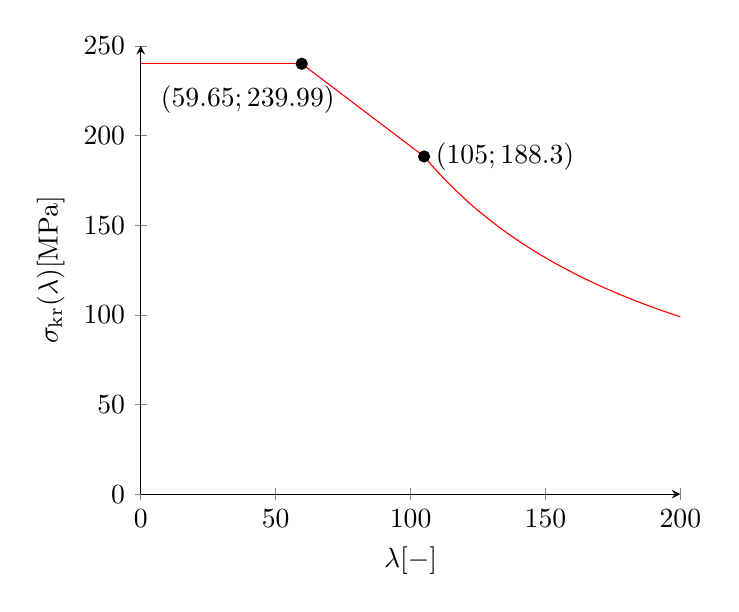
\begin{tikzpicture}
                \begin{axis}[
                        axis lines = left,
			xlabel={$\lambda [-]$},
			ylabel={$\sigma_\text{kr}(\lambda) \mpa{}$},
			ymin=0, ymax=250,
			xmin=0, xmax=200
                ]
                        \addplot [
                                domain=0:59.65,
                                red
                        ]
                                {240};
                        \addplot [
                                domain=59.65:105,
                                red
                        ]
                                {308-1.14*x};
                        \addplot [
                                domain=105:200,
                                red
                        ]
				{19771.5/x};
			\addplot[only marks, mark=*] coordinates {(59.65, 239.99)};
			\addplot[only marks, mark=*] coordinates {(105, 188.3)};
			\node at (59.65 -20, 239.99 -20) {$(59.65; 239.99)$};
			\node at (105 + 30, 188.3) {$(105; 188.3)$};
                \end{axis}
        \end{tikzpicture}
\end{center}

\newpage

\subsection{Minimális falvastagság}
A minimális falvastagság számítása függ attól épp melyik tartományba esik a rúd amit csak a falvastagságból tudnánk, ezért feltételezzük hogy a rúd az Euler-tartományba esik karcsúság szempontjából. A $c$ szorzó az egyenértékű hosszhoz abból származik hogy a rúd alul be van fogva, felül pedig nincs akadályozva a kihajlás.

\begin{align*}
	c &= 2 \\
	h_0 &= ch = \m{5} \\
	F_t = 3\left|B_z\right| &= \left(\frac{\pi}{h_0}\right)^2 I_2 E 
\end{align*}

A keresztmetszet másodrendű nyomatéka függ a geometriától.
\begin{align*}
	I_2 &= \frac{d^4 \pi}{64} - \frac{(d-2t_\text{min})^4 \pi}{64} \\
	t_\text{min} &= 2.49254 \approx \mm{2.5}
\end{align*}

\begin{align*}
	A &= \frac{\left[d^2 - (d-2t_\text{min})^2\right] \pi}{4} \\
	i_2 &= \sqrt{\frac{I_2}{A}} \\ \\
	\lambda &= \frac{h_0}{i_2} = 254.886
\end{align*}
A karcsúság az Euler-tartományba esik, tehát feltételezésünk beigazolódott.

	\newpage

	\section{Nyúlásmérés}

\subsection{Alakváltozási tenzor}
\begin{align*}
	\epsilon_x &= \epsilon_a \\
	\epsilon_z &= \epsilon_c \\
	\epsilon_y &= -\frac{\nu}{1-\nu}(\epsilon_x + \epsilon_z)
\end{align*}

\begin{equation*}
	\pmb{\epsilon} = \begin{bmatrix}
		\epsilon_x & 0 & \frac{1}{2}\gamma_{xz} \\
		0 & \epsilon_y & 0 \\
		\frac{1}{2}\gamma_{zx} & 0 & \epsilon_z \\
	\end{bmatrix} = \begin{bmatrix}
		\num{-5.2e-4} & 0 & \num{-3.4e-4} \\
		0 & \num{9.42857e-5} & 0 \\
		\num{-3.4e-4} & 0 & \num{3e-4} \\
	\end{bmatrix}
\end{equation*}

\begin{equation*}
	\epsilon_\text{I} = \frac{\Delta V}{V} = \text{tr}(\pmb{\epsilon}) = \epsilon_x + \epsilon_y + \epsilon_z = \num{-1.257143e-4}
\end{equation*}

\newpage

\subsection{Hooke-törvény}

\begin{equation*}
	\pmb{\sigma} = \begin{bmatrix}
		\sigma_x & 0 & \tau_{xz} \\
		0 & 0 & 0 \\
		\tau_{zx} & 0 & \sigma_z
	\end{bmatrix} = \frac{E}{1+\nu}\left(\pmb{\epsilon} + \frac{\nu}{1-2\nu} \epsilon_I \pmb{E}\right)
\end{equation*}

\begin{align*}
	\sigma_x &= \frac{E}{1-2\nu}\left(\epsilon_x + \frac{\nu}{1-2\nu} \epsilon_I\right) \\
	\sigma_z &= \frac{E}{1-2\nu}\left(\epsilon_z + \frac{\nu}{1-2\nu} \epsilon_I\right) \\
	\tau_{xz} &= \tau_zx = \frac{E}{1+\nu} \frac{1}{2}\gamma_xz
\end{align*}

\begin{equation*}
	\pmb{\sigma} = \begin{bmatrix}
		-99.231 & 0 & -54.9231 \\
		0 & 0 & 0 \\
		-54.9231 & 0 & 33.231
	\end{bmatrix} \left[\si{\mega\pascal}\right]
\end{equation*}

\begin{center}
	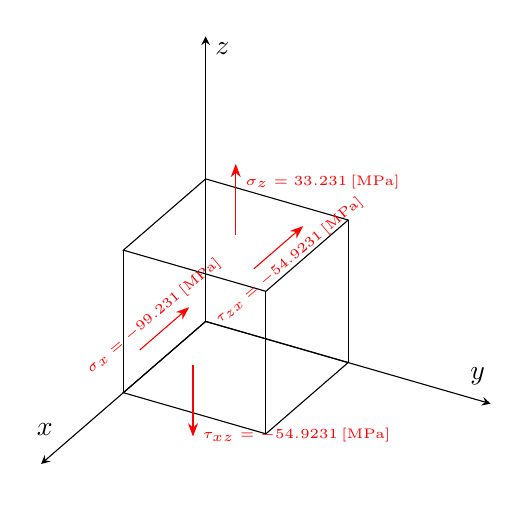
\begin{tikzpicture}
		\begin{axis}[
			view={120}{30},
			width=\textwidth,
			clip=false,
			axis lines=center, 
			xlabel={$x$}, ylabel={$y$}, zlabel={$z$},
			axis equal image,
			xmin=0, xmax=2,
			ymin=0, ymax=2,
			zmin=0, zmax=2,
			xticklabel=\empty,
			yticklabel=\empty,
			zticklabel=\empty,
			tick style={draw=none}
			]
			\addplot3[black] coordinates {(0,0,0) (1,0,0) (1,1,0) (0,1,0) (0,0,0)};
			\addplot3[black] coordinates {(0,0,1) (1,0,1) (1,1,1) (0,1,1) (0,0,1)};
			\addplot3[black] coordinates {(0,0,0) (0,0,1)};
			\addplot3[black] coordinates {(1,0,0) (1,0,1)};
			\addplot3[black] coordinates {(1,1,0) (1,1,1)};
			\addplot3[black] coordinates {(0,1,0) (0,1,1)};

			\addplot3[red, -Stealth] coordinates {(.8, 0, .2) (.2, 0, .2)} node[midway, above, font=\tiny, rotate=40] {$\sigma_x = \mpa{-99.231}$};
			\addplot3[red, -Stealth] coordinates {(.5, .5, 1) (.5, .5, 1.5)} node[near end, right, font=\tiny, rotate=0] {$\sigma_z = \mpa{33.231}$};
			\addplot3[red, -Stealth] coordinates {(.8, .8, 1) (.2, .8, 1)} node[midway, below, font=\tiny, rotate=40] {$\tau_{zx} = \mpa{-54.9231}$};
			\addplot3[red, -Stealth] coordinates {(.5, .2, 0) (.5, .2, -.5)} node[near end, below right, font=\tiny] {$\tau_{xz} = \mpa{-54.9231}$};
		\end{axis}
	\end{tikzpicture}
\end{center}

\begin{align*}
	\sigma_\text{I} &= \text{tr}(\pmb{\sigma}) = \mpa{-66} \\
	\sigma_\text{II} &= \sigma_x \sigma_y + \sigma_x \sigma_z + \sigma_y \sigma_z - \tau_{xy}^2 - \tau_{xz}^2 - \tau_{yz}^2 \\&= \SI{-6314.092275}{[\mega\pascal^2]}\\
	\sigma_\text{III} &= \text{det}(\pmb{\sigma}) = 0
\end{align*}

	\newpage

	\section{Főfeszültségek}

\subsection{Mohr-féle diagram}

\begin{align*}
	\tau_{xy} = \tau_{yz} = 0 &\Rightarrow \sigma_y = 0 \\
				  &\Rightarrow \pmb{e_2} = \begin{bmatrix}
		0 \\
		1 \\
		0
	\end{bmatrix} \\ 
				  &\Rightarrow \sigma_2 = 0
\end{align*}

\begin{align*}
	&X(\sigma_x; \left[\tau_{xz}\right]) = (-99.231; 54.9231) \\
    	&Y(\sigma_y; 0) = (0; 0) \\
	&Z(\sigma_z; \left[\tau_{xz}\right]) = (33.231; 54.9231) \\
\end{align*}

\begin{align*}
	\sigma_\text{K} &= \frac{\sigma_x + \sigma_z}{2} = \mpa{-33} \\
	R &= \sqrt{\left(\frac{\sigma_x - \sigma_z}{2}\right)^2 + \tau_{xz}^2} = \mpa{86.04122}
\end{align*}

\begin{align*}
	\sigma_{1;3} = \sigma_\text{K} \pm R = \begin{cases}
		53.04122 \\
		-119.04122
	\end{cases}
\end{align*}

\begin{center}
	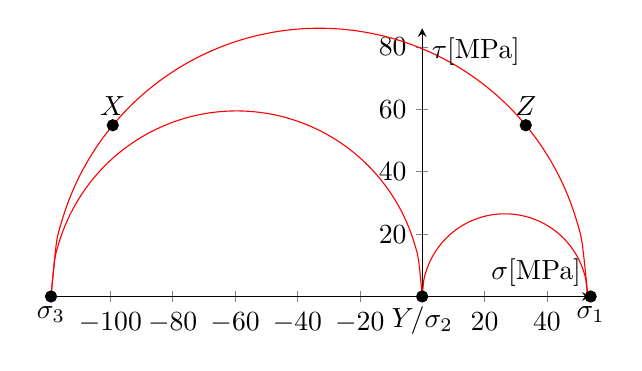
\begin{tikzpicture}
		\begin{axis}[
			axis lines=middle,
			clip=false,
			axis equal image,
			xlabel = {$\sigma \mpa{}$},
			ylabel = {$\tau \mpa{}$},
		]
		\addplot[only marks, mark=*] coordinates {(-99.231, 54.9231)} node [above] {$X$};
		\addplot[only marks, mark=*] coordinates {(0,0)} node [below] {$Y / \sigma_2$};
		\addplot[only marks, mark=*] coordinates {(33.231, 54.9231)} node [above] {$Z$};

		\addplot[only marks, mark=*] coordinates {(-119.04122, 0)} node [below] {$\sigma_3$};
		\addplot[only marks, mark=*] coordinates {(54.04122, 0)} node [below] {$\sigma_1$};

		\addplot[domain=-119.04122:53.04122, samples=100, smooth, red] {sqrt((86.04122)^2-(x + 33)^2)};
		\addplot[domain=-119.04122:0, samples=100, smooth, red] {sqrt((59.52061)^2-(x + 59.52061)^2)};
		\addplot[domain=0:53.04122, samples=100, smooth, red] {sqrt((26.52061)^2-(x - 26.52061)^2)};
		\end{axis}
	\end{tikzpicture}
\end{center}

\subsection{Főirányok}
\begin{align*}
	\phi_1 &= \text{arctg}(\frac{\sigma_1 - \sigma_x}{\tau_{xz}}) = \ang{70.166} \\
	\pmb{e_1} &= \begin{bmatrix}
		\cos \phi_1 \\
		0 \\
		-\sin \phi_1
		\end{bmatrix} = \begin{bmatrix}
			0.3393 \\
			0 \\
			-0.941
		\end{bmatrix} \\
	\pmb{e_3} &= \pmb{e_1} \times \pmb{e_2} = \begin{bmatrix}
		0.941 \\
		0 \\
		0.3393
	\end{bmatrix}
\end{align*}

\subsection{Ellenőrzés}

\subsubsection{Sajátérték}
\begin{align*}
	\text{det}(\pmb{\sigma} - \lambda\pmb{E}) &= 0 \\
	\begin{bmatrix}
		\sigma_x - \lambda & 0 & 0 \\
		0 & -\lambda & 0 \\
		\tau_{xz} & 0 & \lambda_z - \lambda
	\end{bmatrix} &= 0 \\
	(-\lambda)\left[(\sigma_x - \lambda)(\sigma_z - \lambda) - \tau_{xz}^2\right] &= 0 \\ \\
	\lambda_{1;2;3} &= \begin{cases}
		53.04122 \\
		0 \\
		-119.04122
	\end{cases} \\&= \sigma_{1;2;3} \; \checkmark
\end{align*}

\subsubsection{Sajátvektor}
\begin{align*}
	\pmb{\sigma} - \lambda_1 \pmb{E} &= \pmb{0} \\
	\begin{bmatrix}
		\sigma_x - \sigma_1 & 0 & \tau_{xz} \\
		0 & 0 & 0 \\
		\tau_{xz} & 0 & \sigma_z - \sigma_1 
	\end{bmatrix} \begin{bmatrix}
		\cos \phi \\
		0 \\
		\sin \phi
	\end{bmatrix} &= \pmb{0} \\
\end{align*}

\begin{align*}
	(\sigma_x - \sigma_1)\cos \alpha + \tau_{xz} \sin \alpha &= 0 \\
	 \tau_{xz} \cos \alpha + (\sigma_z - \sigma_1)\sin \alpha &= 0 \\
\end{align*}

\begin{align*}
	 \frac{\cos \alpha}{\sin \alpha} &= -\frac{\sigma_z - \sigma_1 + \tau_{xz}}{\sigma_x - \sigma_1 + \tau_{xz}} \\
	 \alpha &= \ang{70.1661} = \phi \checkmark
\end{align*}


	\newpage

	\section{Pontbeli feszültségi állapot}

\begin{align*}
	\sigma_e^\text{Mohr} &= \sigma_1 - \sigma_3 = \mpa{172.08244}  \\
	\sigma_e^\text{HMH} &= \sqrt{\frac{1}{2}\left[(\sigma_1 - \sigma_2)^2 + (\sigma_1 - \sigma_3)^2 + (\sigma_2 - \sigma_3)^2\right]} = \mpa{152.6377}
\end{align*}
	
\begin{equation*}
	\Delta \sigma_e = \sigma_e^\text{Mohr} - \sigma_e^\text{HMH} = \mpa{19.445}
\end{equation*}

	\newpage

	\section{Pontbeli alakváltozási energiasűrűség}

\begin{equation*}
	u = \frac{1}{2}\pmb{\sigma}:\pmb{\epsilon} = \SI{0.04946}{[\joule\per\centi\meter^3]} \\
\end{equation*}

\begin{align*}
	\pmb{\epsilon_I} &= \frac{1}{3}\epsilon_I\pmb{E} \\
	\pmb{\sigma} &= \frac{1}{3}\sigma_I\pmb{E} \\
	u_h = \frac{1}{2}\pmb{\sigma_I}:\pmb{\epsilon_I} &= \frac{1}{6} \sigma_I \epsilon_I = \num{1.3828573e-3}
\end{align*}

\begin{equation*}
	u_d = u - u_h = \SI{0.0481}{[\joule\per\centi\meter^3]} \\
\end{equation*}

	\newpage
\end{document}
